\section{User Study 1}

\begin{enumerate}
\item Process of gameplay
\item User's feedback for existing games
\item User's imagination
\end{enumerate}

In order to realize the current game play experience on google glass. We use games currently existing on google glass to perform our user study. Furthermore, with a view to understanding the response and feedback for different control style and game content from users, we choose four games, ``Balance'', ``Shape Splitter'', ``Matcher'', and ``Clay Shooter'', with unique control type respectively(see Table~\ref{tab:gameControlTypes}).

About our process, we gave user five minutes to play each game, and filled in a questionnaire after playing each game. To make results effective, the order of the game were counterbalanced to eliminate the effects of ordering. After playing all four games, we also provided a final questionnaire to realize the whole glass game play experience from users.


\begin{table}[!h]
\newcommand{\tabincell}[2]{\begin{tabular}{@{}#1@{}}#2\end{tabular}}
   \centering
   \begin{tabular}{|p{0.4\columnwidth}|p{0.4\columnwidth}|}
     \hline
     % \tabhead{Objects} &
     \multicolumn{1}{|p{0.3\columnwidth}|}{\centering\tabhead{Game}} &
     \multicolumn{1}{|p{0.5\columnwidth}|}{\centering\tabhead{Control}} \\
     \hline
     Balance & gyro\\
     \hline
     Shape Splitter & in-air gesture\\
     \hline
     Matcher & gyro, tap\\
     \hline
     Clay Shooter & gyro, voice control\\
     \hline
   \end{tabular}
   \caption{Game control types}
   \label{tab:gameControlTypes}
 \end{table}



\subsection{User feedback}
Focusing on Glass too long is not comfortable
Gyro is comfortable for 1D and 2D control
Gyro with 360 degree is BAD
Voice Control \& In-Air Gesture are NOT social acceptable
tapping is acceptable many tappings are annoying
In air gesture is tiring
Current in air gesture detecting sucks
Voice control always out of control



\begin{table}[!h]
\newcommand{\tabincell}[2]{\begin{tabular}{@{}#1@{}}#2\end{tabular}}
   \centering
   \begin{tabular}{|p{0.4\columnwidth}|p{0.3\columnwidth}|}
     \hline
     % \tabhead{Objects} &
     \multicolumn{1}{|p{0.3\columnwidth}|}{\centering\tabhead{Category}} &
     \multicolumn{1}{|p{0.5\columnwidth}|}{\centering\tabhead{User Feedback}} \\
     \hline
     Focusing on Glass too long is not comfortable & \tabincell{c}{p1: hihi I'm p1. I'm feedback.\\p2: hihi I'm p2. I'm feedback2.} \\
     \hline
     Gyro is comfortable for 1D and 2D control & \\
     \hline
     Gyro with 360 degree is BAD & \\
     \hline
     Voice Control \& In-Air Gesture are NOT social acceptable & \\
     \hline
     tapping is acceptable many tappings are annoying & \\
     \hline
     In air gesture is tiring & \\
     \hline
     Current in air gesture detecting sucks & \\
     \hline
     Voice control always out of control & \\
     \hline
   \end{tabular}
   \caption{Small Sun.}
   \label{tab:table1}
 \end{table}

 \begin{table}[!h]
\newcommand{\tabincell}[2]{\begin{tabular}{@{}#1@{}}#2\end{tabular}}
   \centering
   \begin{tabular}{|p{0.4\columnwidth}|p{0.3\columnwidth}|}
     \hline
     % \tabhead{Objects} &
     \multicolumn{1}{|p{0.3\columnwidth}|}{Game Play Feedback} &
     \multicolumn{1}{|p{0.5\columnwidth}|}{Level design, Music, Visual art, Casual, Challenge, Game for purpose, Innovative, Physics, Immersion} \\
     % \multicolumn{1}{|p{0.3\columnwidth}|}{\centering\tabhead{Game Play Feedback}} &
     % \multicolumn{1}{|p{0.5\columnwidth}|}{\centering\tabhead{User Feedback}} \\
     \hline
     \multicolumn{1}{|p{0.3\columnwidth}|}{Glass Related Feedback} & 
     \multicolumn{1}{|p{0.5\columnwidth}|}{Gyro, In-air gesture, Tap, Voice control, Eye tiring, Social acceptable, AR} \\
     \hline
   \end{tabular}
   \caption{We collect 304 feedbacks and manually divide into 16 categories.}
   \label{tab:table1}
 \end{table}

% \begin{table}
% \newcommand{\tabincell}[2]{\begin{tabular}{@{}#1@{}}#2\end{tabular}}
%   \centering
%   \begin{tabular}{|c|c|c|}\hline
% 1 & \tabincell{c}{the first line \\ the next\\the next\\ last} & \tabincell{c}{one \\ one}\\\hline
% 2 & \tabincell{c}{hello\\ aha\\ ok \\yes \\en} & \tabincell{c}{two \\ two \\ two} \\\hline
% \end{tabular}
%   \caption{longtitle}
% \end{table}

\begin{figure}[!t]
\centering
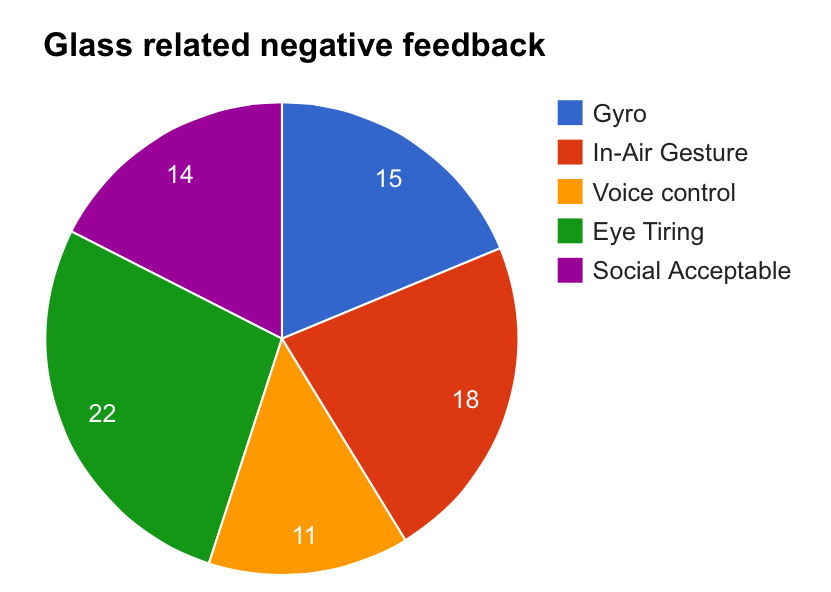
\includegraphics[width=0.9\columnwidth]{Figures/US1_userfeedbackStatistics.png}
\caption{Hi I'm Small Sun.}
\label{fig:PS_Frus}
\end{figure}


\subsection{Observation}

\begin{enumerate}
\item NOT social acceptable != NOT fun
\item Small movement is better
\end{enumerate}


\subsection{User imagination}

\begin{figure}[!t]
\centering
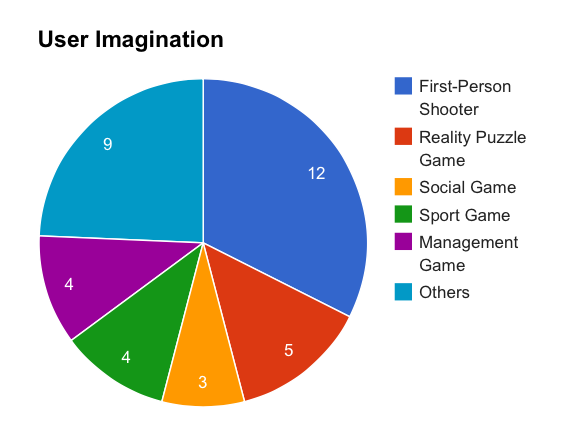
\includegraphics[width=0.9\columnwidth]{Figures/US1_userImaginationStatistics.png}
\caption{Hi I'm Small Sun 2.}
\label{fig:PS_Frus}
\end{figure}
